This test problem is the classic 1-D dam break problem for the shallow
water equations \cite{leveque2002}. This is an example of a Riemann problem
for the SWE: the initial data consists of constant left and right states.
The problem parameters are summarized in Table \ref{tab:dam_break_1d}.

%-------------------------------------------------------------------------------
\begin{table}[htb]\caption{Bathtub Test Problem Summary}
\label{tab:dam_break_1d}
\centering
\begin{tabular}{l l}\toprule
\emph{Parameter} & \emph{Value}\\\midrule
Domain & $\mathcal{D} = (0,1)^2$\\
Initial Conditions & $\height_0(\x)=1 + e^{-250((x-0.25)^2+(y-0.25)^2)}$\\
                   & $\velocity_0(\x) = \mathbf{0}$\\
Boundary Conditions & $\nabla\height(\x,t)=0
  \eqc \quad \x\in\partial\mathcal{D}\eqc \quad t>0$,\\
                    & $\velocity\xt\cdot\normalvector = 0
  \eqc \quad \x\in\partial\mathcal{D}\eqc \quad t>0$,\\
Bathymetry & $\bathymetry(\x)=0$\\
Gravity    & $\gravity=1$\\
\bottomrule\end{tabular}
\end{table}
%-------------------------------------------------------------------------------

The simulations were run using a CFL of 0.1 to a final time of $t=2$,
using explicit Euler and SSPRK33.
For the entropy viscosity method, the entropy residual coefficient
and entropy jump coefficient were set to $\entropyresidualcoef=1$
and $\entropyjumpcoef=1$, respectively.
Figures \ref{fig:height_FE_32} and \ref{fig:momentum_FE_32} 
show the height and momentum solutions, respectively, obtained using explicit Euler
and 32 cells, and Figures \ref{fig:height_FE_256} and \ref{fig:momentum_FE_256} 
show the solutions for 256 cells.

%-------------------------------------------------------------------------------
\begin{figure}[ht]
   \centering
   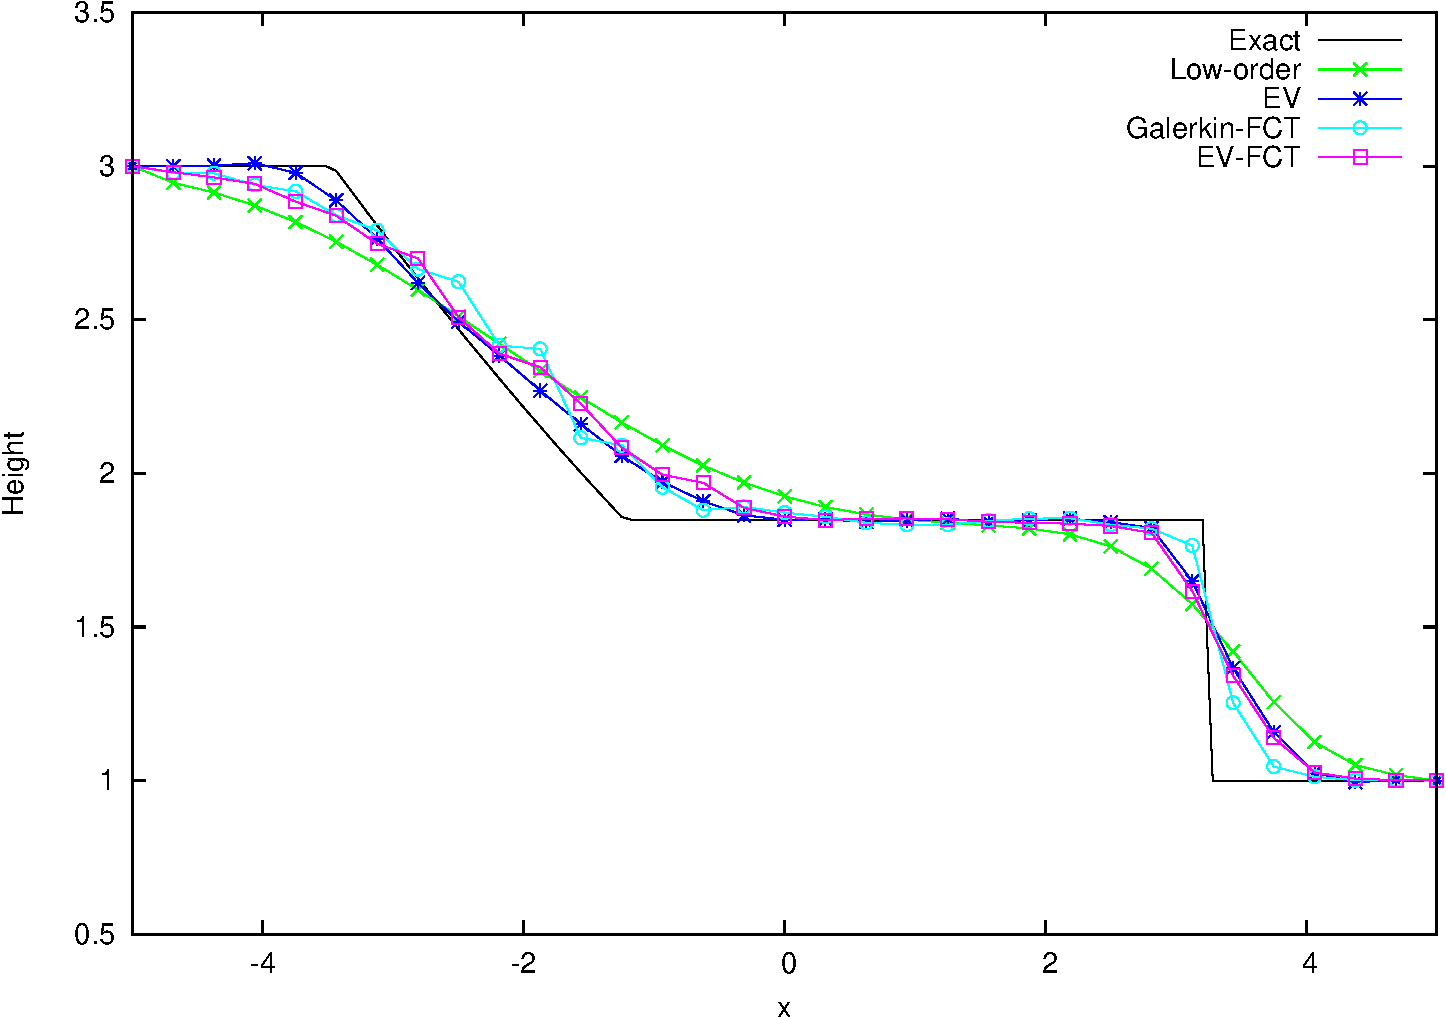
\includegraphics[width=\textwidth]
     {\contentdir/results/shallowwater/dam_break_1d/images/Height_FE_32cells.pdf}
   \caption{Comparison of Height Solutions for the 1-D Dam Break Test Problem
     Using Explicit Euler with 32 cells}
   \label{fig:height_FE_32}
\end{figure}
%-------------------------------------------------------------------------------
\begin{figure}[ht]
   \centering
   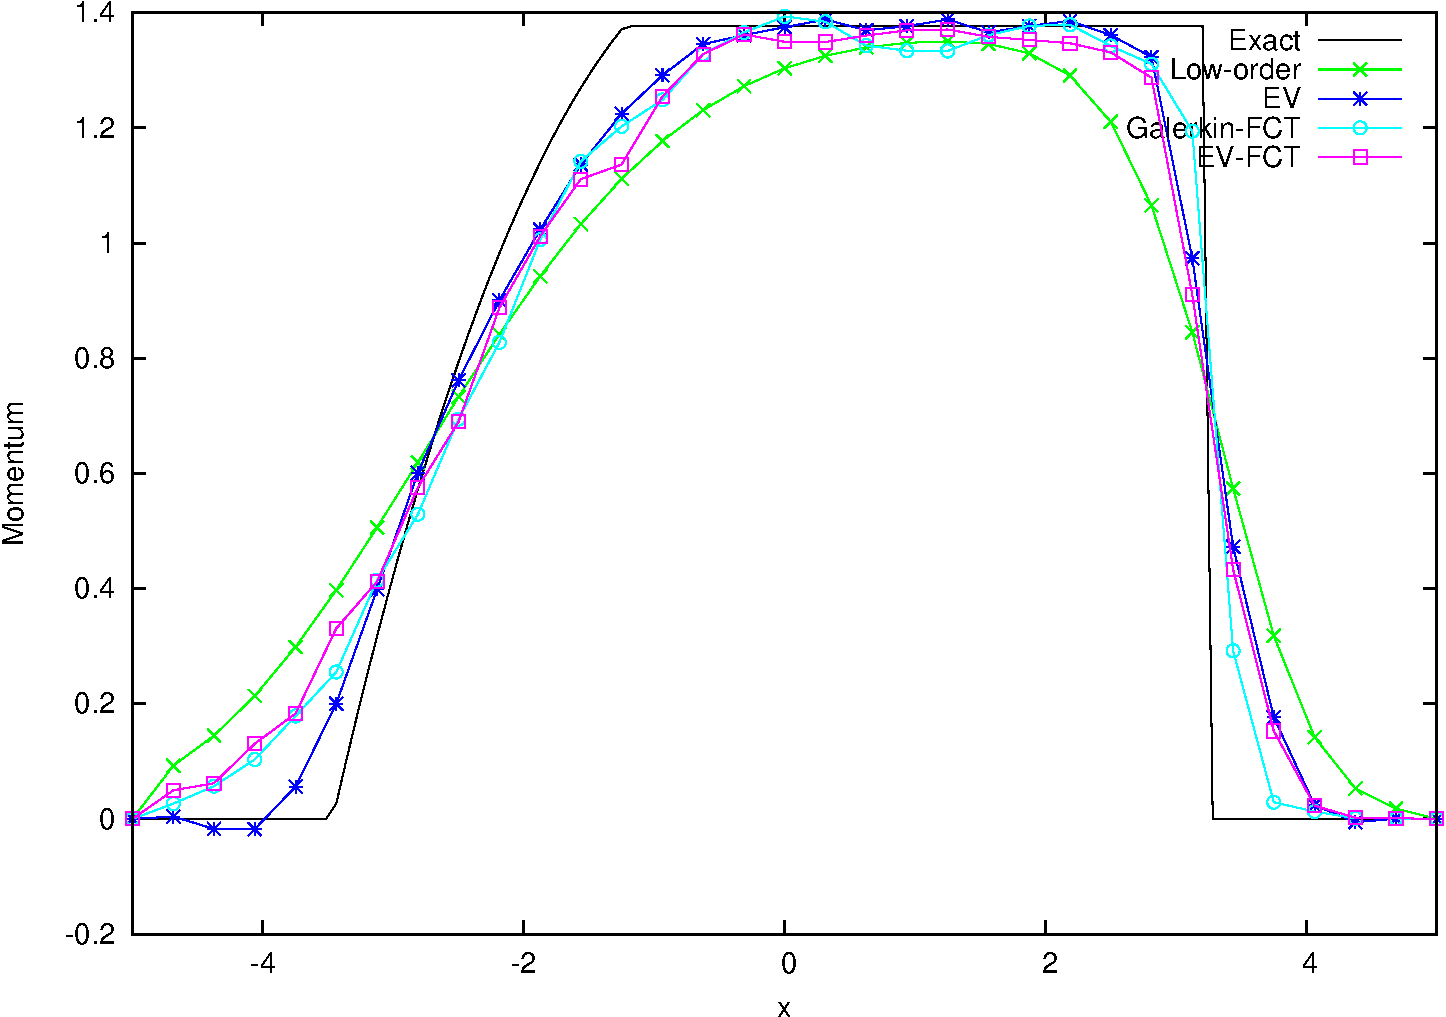
\includegraphics[width=\textwidth]
     {\contentdir/results/shallowwater/dam_break_1d/images/Momentum_FE_32cells.pdf}
   \caption{Comparison of Momentum Solutions for the 1-D Dam Break Test Problem
     Using Explicit Euler with 32 cells}
   \label{fig:momentum_FE_32}
\end{figure}
%-------------------------------------------------------------------------------
\begin{figure}[ht]
   \centering
   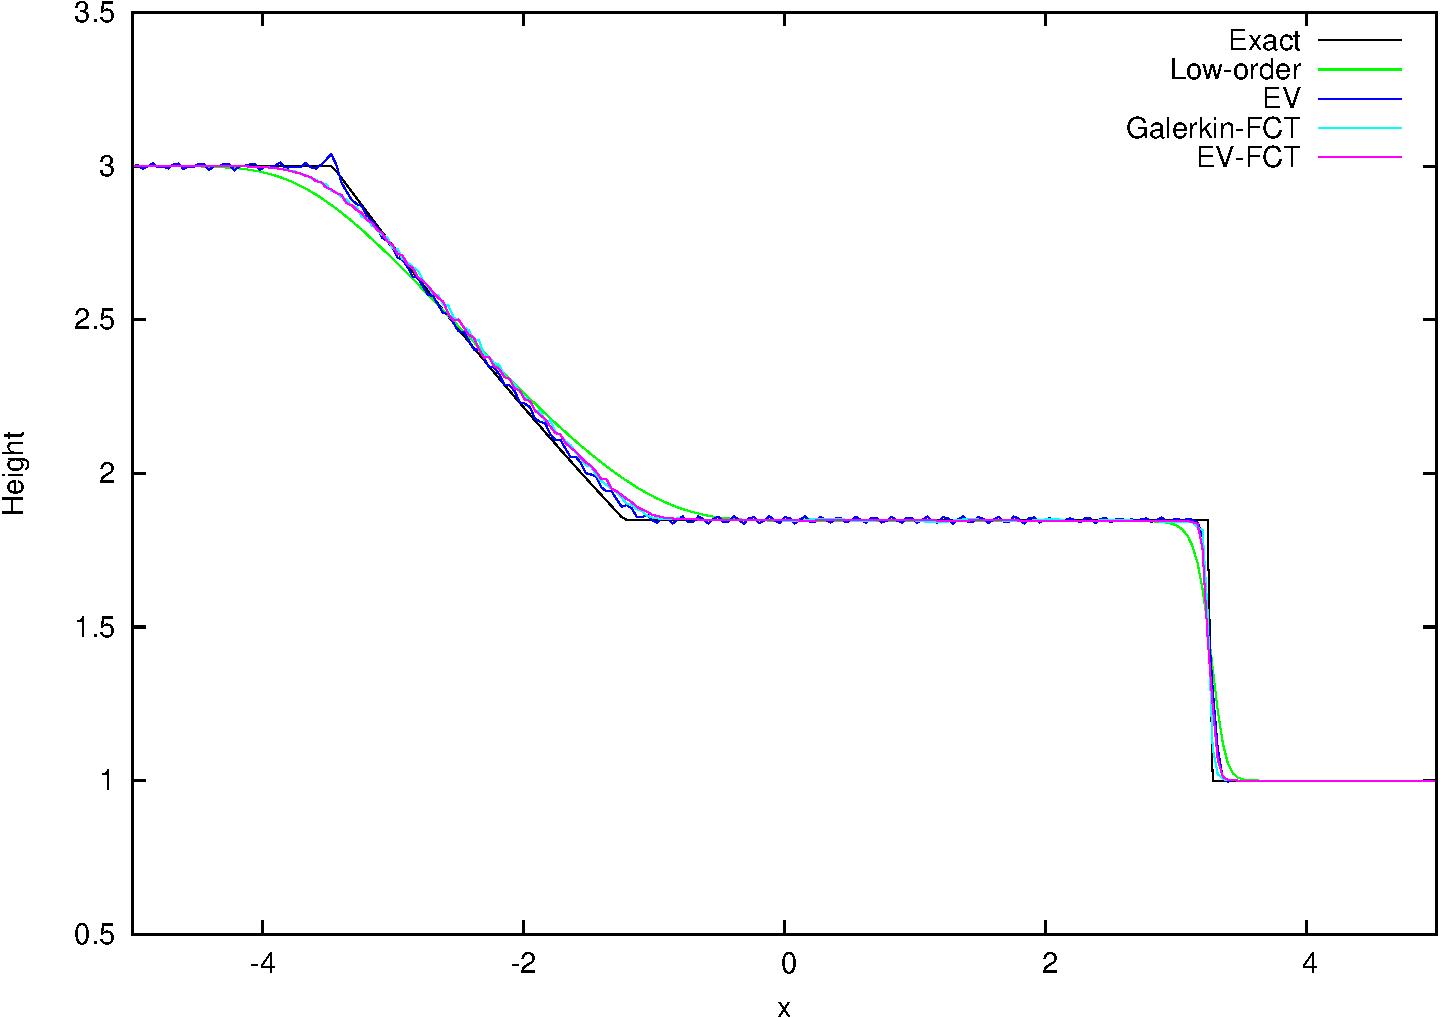
\includegraphics[width=\textwidth]
     {\contentdir/results/shallowwater/dam_break_1d/images/Height_FE_256cells.pdf}
   \caption{Comparison of Height Solutions for the 1-D Dam Break Test Problem
     Using Explicit Euler with 256 cells}
   \label{fig:height_FE_256}
\end{figure}
%-------------------------------------------------------------------------------
\begin{figure}[ht]
   \centering
   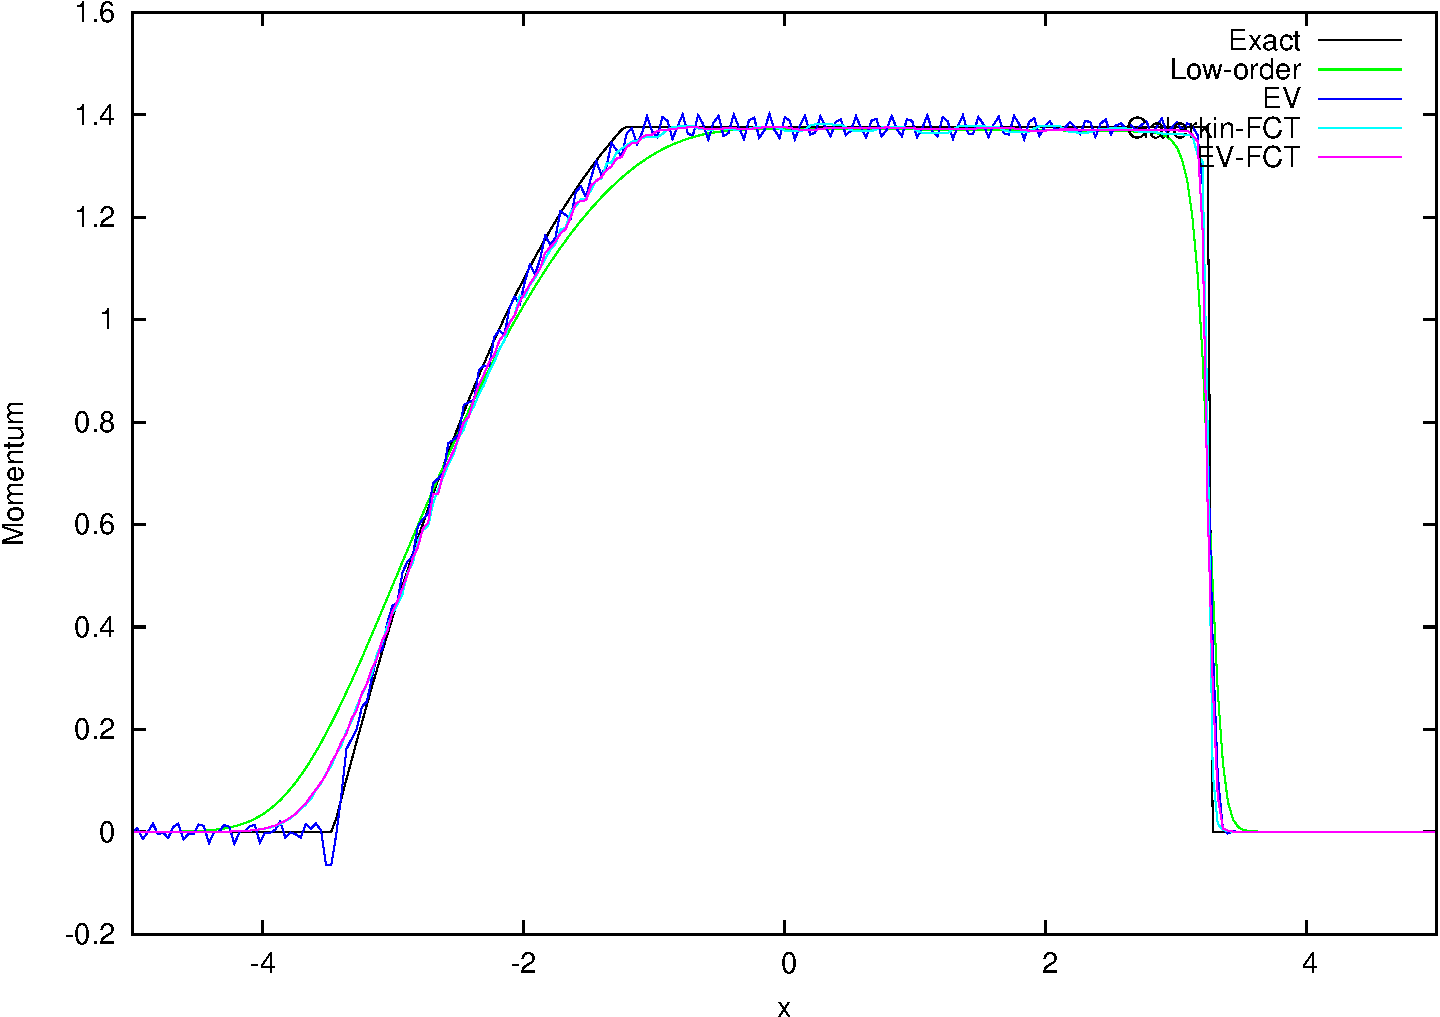
\includegraphics[width=\textwidth]
     {\contentdir/results/shallowwater/dam_break_1d/images/Momentum_FE_256cells.pdf}
   \caption{Comparison of Momentum Solutions for the 1-D Dam Break Test Problem
     Using Explicit Euler with 256 cells}
   \label{fig:momentum_FE_256}
\end{figure}
%-------------------------------------------------------------------------------

\clearpage
